 
\chapter{Dados Obtidos}
\label{cap6}

\begin{figure}[htb!]
    \caption{Tempo de requisição a partir dos Clientes}
    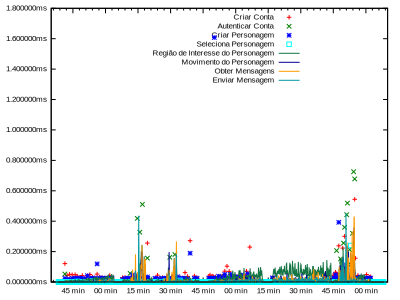
\includegraphics[width=\textwidth]{metricas_rudy_t3/rudyc.png}
    \centering
    
    Fonte: O próprio autor
\end{figure}

\begin{figure}[htb!]
    \caption{Tempo de requisição a partir dos Clientes}
    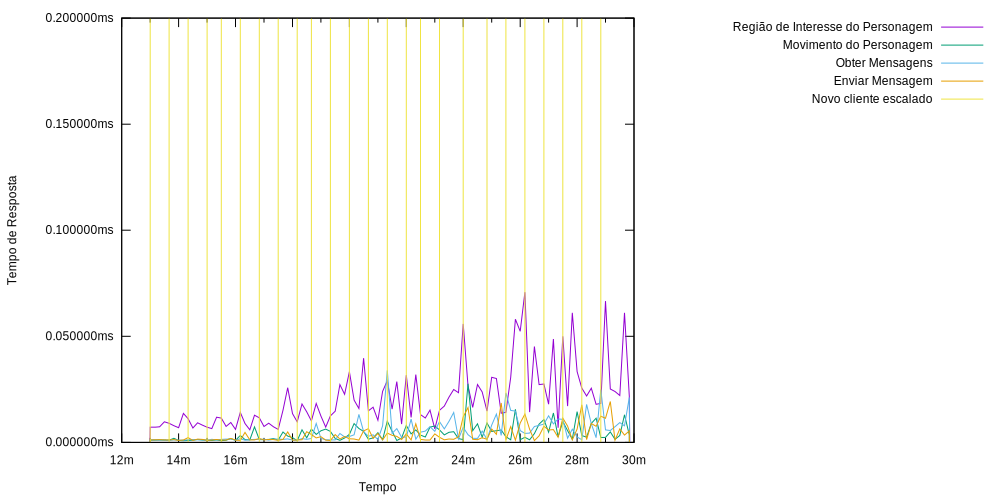
\includegraphics[width=\textwidth]{metricas_rudy_t3/rudyc_rpc.png}
    \centering
    
    Fonte: O próprio autor
\end{figure}

\begin{figure}[htb!]
    \caption{Tempo de requisição a partir dos Clientes}
    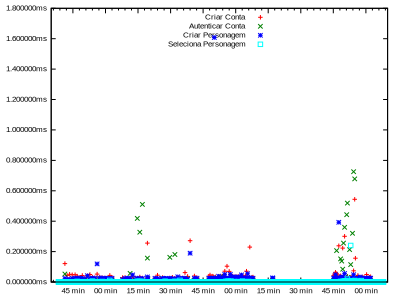
\includegraphics[width=\textwidth]{metricas_rudy_t3/rudyc_http.png}
    \centering
    
    Fonte: O próprio autor
\end{figure}

\begin{figure}[htb!]
    \caption{Tempo de requisição a partir dos Clientes}
    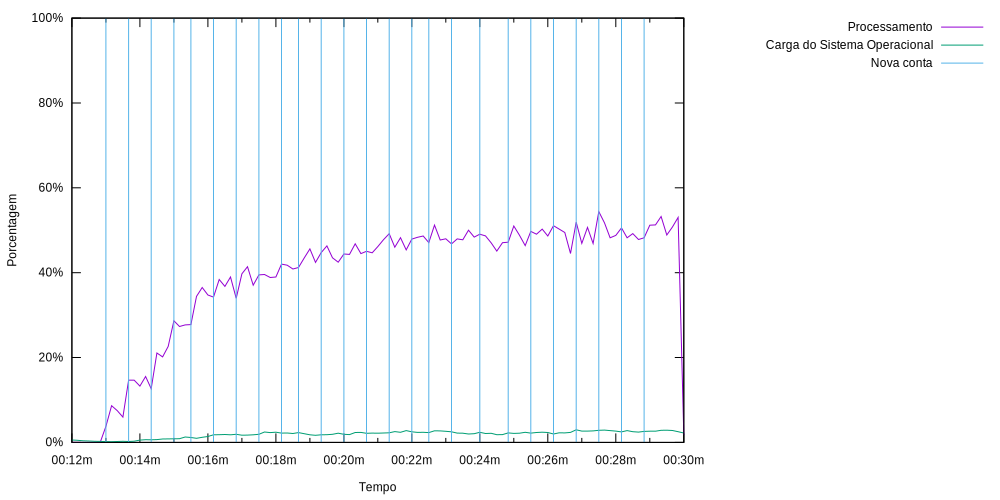
\includegraphics[width=\textwidth]{metricas_rudy_t3/cpu.png}
    \centering
    
    Fonte: O próprio autor
\end{figure}

\begin{figure}[htb!]
    \caption{Tempo de requisição a partir dos Clientes}
    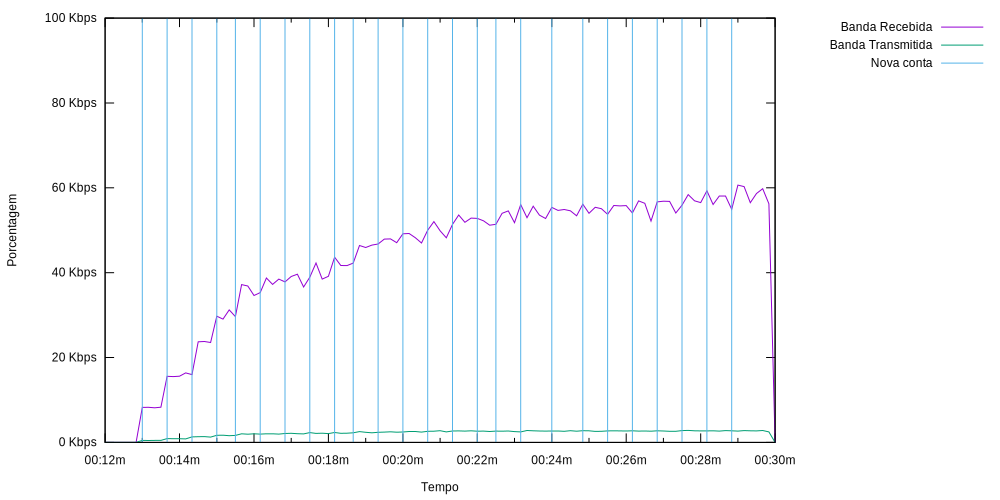
\includegraphics[width=\textwidth]{metricas_rudy_t3/io.png}
    \centering
    
    Fonte: O próprio autor
\end{figure}

\begin{figure}[htb!]
    \caption{Tempo de requisição a partir dos Clientes}
    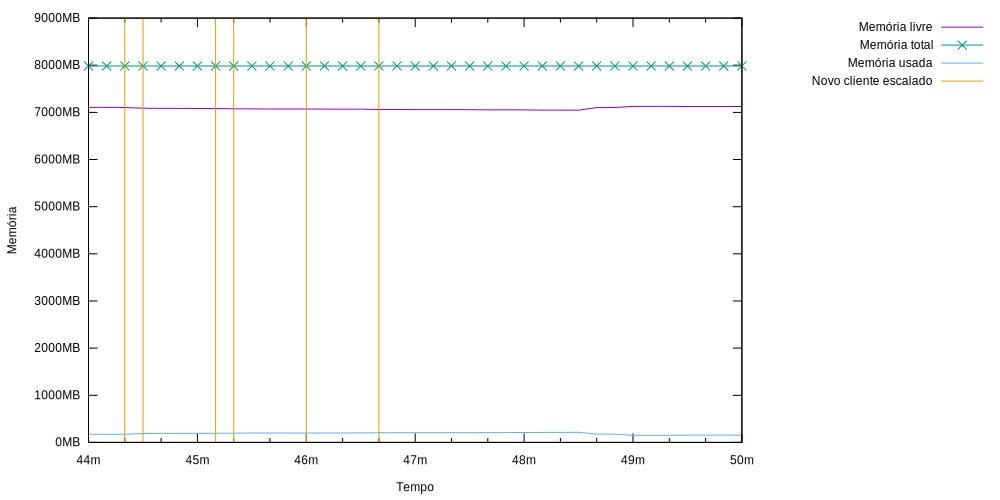
\includegraphics[width=\textwidth]{metricas_rudy_t3/memory.png}
    \centering
    
    Fonte: O próprio autor
\end{figure}